\subsection{Caso d'uso UC0: Monolith.}
\begin{itemize}
   \FloatBarrier
   \begin{figure}[ht]
   \centering
   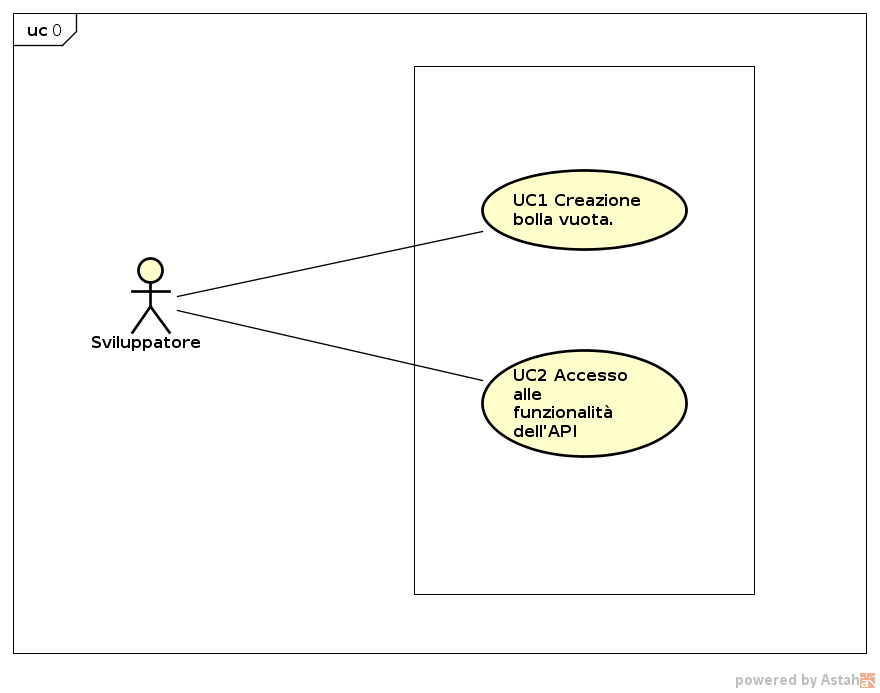
\includegraphics[scale=0.45]{img/UC0.png}
   \caption{Diagramma per il caso d'uso UC0.}
\end{figure}
\FloatBarrier
\item[]\textbf{Descrizione:} Lo sviluppatore ha a disposizione gli strumenti per poter creare una bolla funzionante. Ha la possibilità di inizializzare una bolla nuova o di aggiungere funzionalità offerte dall'API.
\item[]\textbf{Attori:} Sviluppatore. 
\item[]\textbf{Precondizione:} Il sistema è installato e pronto all'uso. 
\item[]\textbf{Postcondizione:} Lo sviluppatore ha avuto modo di utilizzare le funzionalità offerte dall'SDK. 
\item[]\textbf{Scenario:}
\begin{enumerate}


\item Lo sviluppatore ha la possibilità di creare una bolla vuota.(UC1)


\item Lo sviluppatore accede alle funzionalità offerte dal sistema di API (UC2)


\end{enumerate} 
\end{itemize}

\subsection{Caso d'uso UC1: Creazione bolla vuota.}
\begin{itemize}
\item[]\textbf{Descrizione:} Lo sviluppatore sceglie di creare una nuova bolla. Il sistema inizializza una bolla vuota e predispone l'ambiente di lavoro (files di progetto pronti alle modifiche). La parte grafica della bolla include solo un contenitore vuoto d'ora in poi riferito come contenitore principale.
\item[]\textbf{Attori:} Sviluppatore. 
\item[]\textbf{Precondizione:} Il sistema è installato e pronto all'uso. 
\item[]\textbf{Postcondizione:} La bolla vuota è stata creata. 
\item[]\textbf{Scenario:}
Lo sviluppatore sceglie di eseguire la procedura di inizializzazione per una nuova bolla e il sistema crea i files necessari. 
\end{itemize}

\clearpage

\subsection{Caso d'uso UC2: Accesso alle funzionalità dell'API.}
\begin{itemize}
   \FloatBarrier
   \begin{figure}[ht]
   \centering
   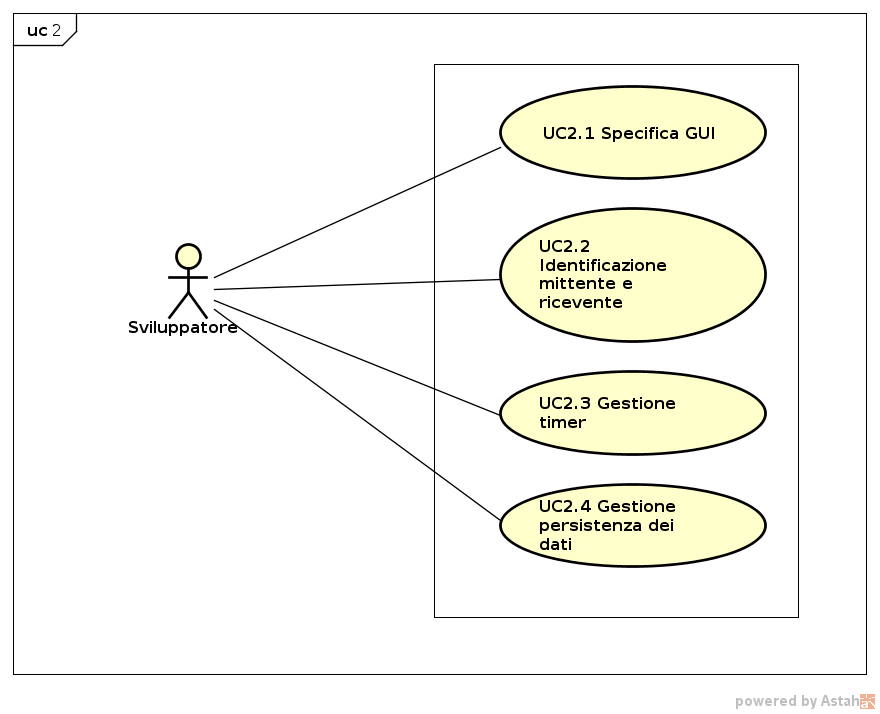
\includegraphics[scale=0.45]{img/UC2.png}
   \caption{Diagramma per il caso d'uso UC2.}
\end{figure}
\FloatBarrier
\item[]\textbf{Descrizione:} Lo sviluppatore utilizza le funzionalità offerte dall'API nella propria bolla.
\item[]\textbf{Attori:} Sviluppatore. 
\item[]\textbf{Precondizione:} Esiste una bolla (vuota o meno). 
\item[]\textbf{Postcondizione:} Lo sviluppatore ha aggiunto alla bolla le funzionalità desiderate. 
\item[]\textbf{Scenario:}
\begin{enumerate}


\item Lo sviluppatore utilizza le funzionalità per determinare la GUI (UC2.1).


\item Lo sviluppatore identifica le tipologie di utente (UC2.2).

\item Lo sviluppatore imposta l'esecuzione a tempo di alcune azioni (UC2.3).

\item Lo sviluppatore gestisce la persistenza dei dati (UC2.4).

\end{enumerate} 
\end{itemize}

\clearpage

\subsection{Caso d'uso UC2.1: Specifica GUI.}
\begin{itemize}
   \FloatBarrier
   \begin{figure}[ht]
   \centering
   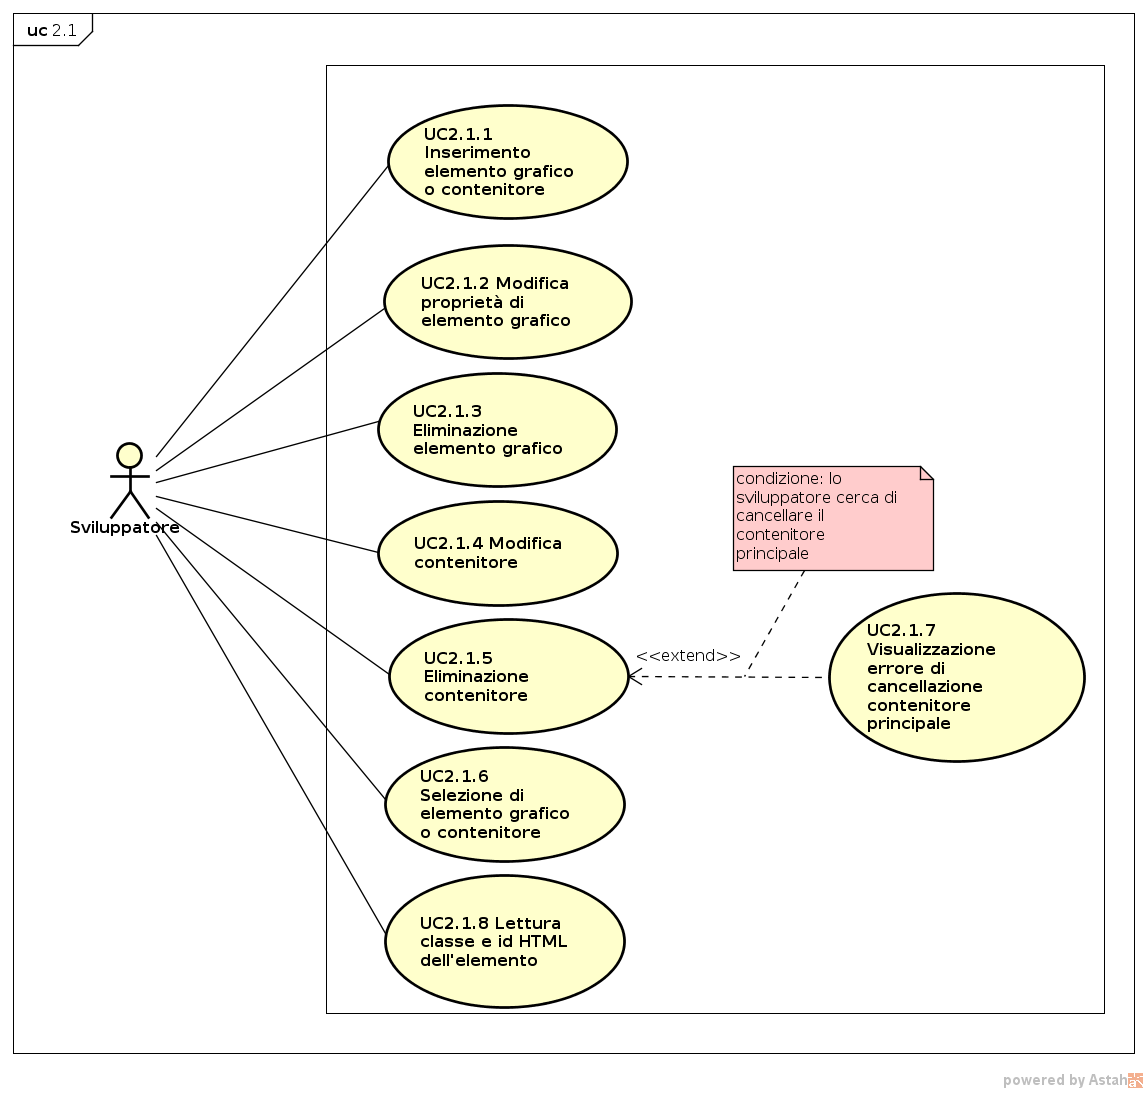
\includegraphics[scale=0.45]{img/UC2_1.png}
   \caption{Diagramma per il caso d'uso UC2.1.}
\end{figure}
\FloatBarrier
\item[]\textbf{Descrizione:} Lo sviluppatore utilizza le funzionalità offerte dall'API per descrivere l'aspetto visuale della bolla.
\item[]\textbf{Attori:} Sviluppatore. 
\item[]\textbf{Precondizione:} Esiste una bolla. 
\item[]\textbf{Postcondizione:} L'aspetto visuale della bolla è stato modificato. 
\item[]\textbf{Scenario:}
\begin{enumerate}


\item Lo sviluppatore inserisce un elemento grafico o un contenire (UC2.1.1).

\item Lo sviluppatore modifica le proprietà di un elemento grafico (UC2.1.2).


\item Lo sviluppatore elimina un elemento grafico (UC2.1.3).

\item Lo sviluppatore modifica le proprietà di un contenitore (UC2.1.4).


\item Lo sviluppatore elimina un contenitore (UC2.1.5).

\item Lo sviluppatore seleziona un elemento grafico o un contenitore (UC2.1.6).

\item Lo sviluppatore visualizza id o classe HTML dell'elemento o contenitore selezionato (UC2.1.8).

\end{enumerate} 
\item[]\textbf{Estensioni:}
Viene visualizzato un messaggio di errore per aver provato a eliminare il contenitore principale (UC2.1.7). 
\end{itemize}

\subsection{Caso d'uso UC2.1.1: Inserimento di un elemento grafico o di un contenitore.}
\begin{itemize}
\item[]\textbf{Descrizione:} Lo sviluppatore inserisce un elemento grafico o un contenitore in un contenitore selezionato.
\item[]\textbf{Attori:} Sviluppatore. 
\item[]\textbf{Precondizione:} La bolla esiste e include almeno un contenitore. \'E stato selezionato il contenitore in cui aggiungere l'elemento. 
\item[]\textbf{Postcondizione:} Alla bolla è stato aggiunto un elemento grafico o un contenitore nel contenitore selezionato. 
\item[]\textbf{Scenario:}
Lo sviluppatore può inserire un contenitore o un elemento grafico tra quelli supportati:


\begin{itemize}

\item Elemento di testo.

\item Elemento immagine.

\item Elemento campo di inserimento testo.

\item Elemento pulsante.

\item Elemento checkbox.

\item Elemento radio button.

\end{itemize}

\'E inoltre possibile inserire elementi realizzati dallo sviluppatore. 
\end{itemize}

\clearpage

\subsection{Caso d'uso UC2.1.2: Modifica proprietà di un elemento grafico.}
\begin{itemize}
   \FloatBarrier
   \begin{figure}[ht]
   \centering
   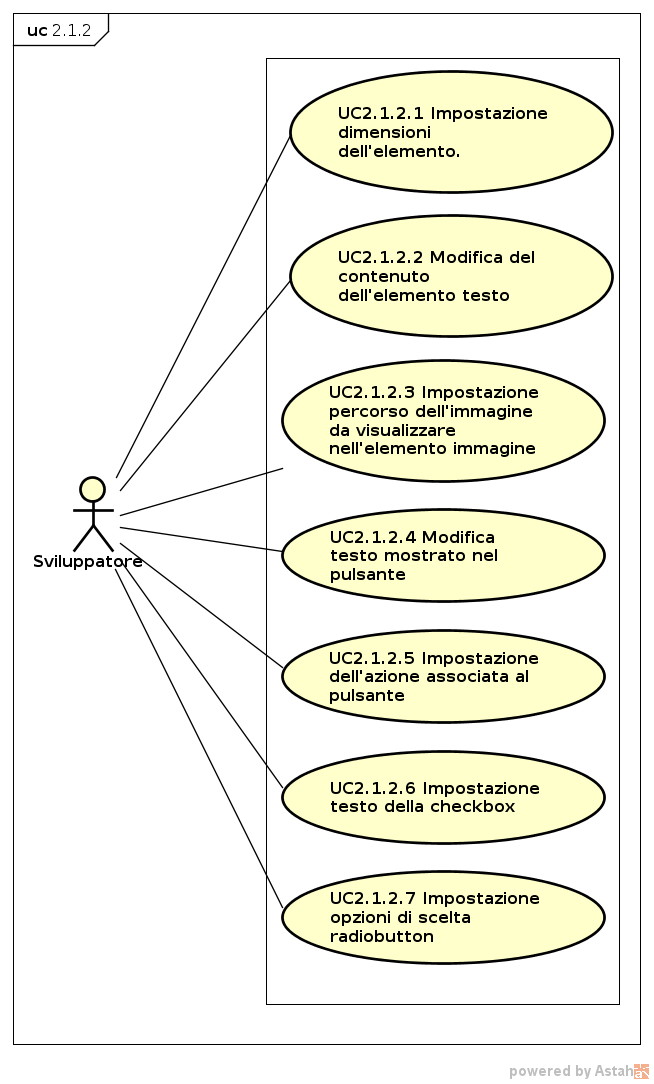
\includegraphics[scale=0.45]{img/UC2_1_2.png}
   \caption{Diagramma per il caso d'uso UC2.1.2.}
\end{figure}
\FloatBarrier
\item[]\textbf{Descrizione:} Gli elementi grafici hanno varie proprietà il cui valore può essere modificato. Alcune proprietà riguardano tutte le tipologie di elemento grafico, altre sono valide solo per alcune. Una volta selezionato l'elemento grafico desiderato l'API permette di modificare il valore di una sua proprietà.
\item[]\textbf{Attori:} Sviluppatore. 
\item[]\textbf{Precondizione:} \'E stato selezionato un elemento grafico. 
\item[]\textbf{Postcondizione:} \'E stata modificata una proprietà dell'elemento grafico. 
\item[]\textbf{Scenario:}
Dopo che l'elemento grafico è stato selezionato (come in UC2.1.6) lo sviluppatore può alterare le sue proprietà:


\begin{enumerate}

\item Impostazione dimensioni dell'elemento(UC2.1.2.1).

\item Modifica del contenuto dell'elemento di testo (UC2.1.2.2).

\item Selezione dell'immagine da visualizzare nell'elemento immagine (UC2.1.2.3).

\item Modifica testo mostrato nel pulsante (UC2.1.2.4).

\item Impostazione dell'azione associata al pulsante (UC2.1.2.5).

\item Impostazione testo della checkbox (UC2.1.2.6).

\item Impostazione opzioni di scelta radiobutton (UC2.1.2.7).

\end{enumerate} 
\end{itemize}

\subsection{Caso d'uso UC2.1.2.1: Impostazione dimensioni dell'elemento.}
\begin{itemize}
\item[]\textbf{Descrizione:} Lo sviluppatore modifica le dimensioni dell'elemento selezionato. Sono possibili due tipi di operazione:

\begin{itemize}

\item lungo la direzione gestita dal contenitore è possibile impostare la dimensione in percentuale sulla dimensione totale. Gli altri eventuali elementi o contenitori saranno distribuiti nello spazio rimanente.


\item Lungo la direzione non gestita dal contenitore è possibile impostare solo dimensioni assolute.


\end{itemize}.
\item[]\textbf{Attori:} Sviluppatore. 
\item[]\textbf{Precondizione:} \'E stato selezionato un elemento grafico. 
\item[]\textbf{Postcondizione:} Le dimensioni dell'elemento grafico  sono state cambiate. 
\item[]\textbf{Scenario:}
Lo sviluppatore ha selezionato un elemento grafico e ne cambia le dimensioni. 
\end{itemize}

\subsection{Caso d'uso UC2.1.2.2: Modifica del contenuto dell'elemento testo.}
\begin{itemize}
\item[]\textbf{Descrizione:} Viene modificato il contenuto dell'elemento di testo selezionato.
\item[]\textbf{Attori:} Sviluppatore. 
\item[]\textbf{Precondizione:} \'E stato selezionato l'elemento di tipo testo da modificare. 
\item[]\textbf{Postcondizione:} Il contenuto dell'elemento testo è stato modificato. 
\item[]\textbf{Scenario:}
Lo sviluppatore modifica il contenuto dell'elemento di testo precedentemente selezionato. 
\end{itemize}

\subsection{Caso d'uso UC2.1.2.3: Impostazione percorso dell'immagine da visualizzare nell'elemento immagine.}
\begin{itemize}
\item[]\textbf{Descrizione:} Viene impostato il percorso dell'immagine da visualizzare nell'elemento.
\item[]\textbf{Attori:} Sviluppatore. 
\item[]\textbf{Precondizione:} \'E stato selezionato un elemento di tipo immagine. 
\item[]\textbf{Postcondizione:} \'E stata impostata la sorgente dell'immagine da visualizzare. 
\item[]\textbf{Scenario:}
Lo sviluppatore imposta il percorso dell'immagine da visualizzare. 
\end{itemize}

\subsection{Caso d'uso UC2.1.2.4: Modifica testo mostrato nel pulsante.}
\begin{itemize}
\item[]\textbf{Descrizione:} Viene modificato il testo mostrato all'interno di un elemento pulsante precedentemente selezionato.
\item[]\textbf{Attori:} Sviluppatore. 
\item[]\textbf{Precondizione:} \'E stato selezionato un elemento di tipo pulsante. 
\item[]\textbf{Postcondizione:} Il testo mostrato nel pulsante è stato modificato. 
\item[]\textbf{Scenario:}
Lo sviluppatore modifica il testo mostrato all'interno di un pulsante. 
\end{itemize}

\subsection{Caso d'uso UC2.1.2.5: Impostazione dell'azione associata al pulsante.}
\begin{itemize}
\item[]\textbf{Descrizione:} Viene impostata l'azione che il sistema deve eseguire quando l'utente preme il pulsante.
\item[]\textbf{Attori:} Sviluppatore. 
\item[]\textbf{Precondizione:} \'E stato selezionato un elemento di tipo pulsante. 
\item[]\textbf{Postcondizione:} L'azione associata al pulsante è stata impostata. 
\item[]\textbf{Scenario:}
Lo sviluppatore imposta l'azione che il sistema deve intraprendere quando l'utente preme il pulsante selezionato. 
\end{itemize}

\subsection{Caso d'uso UC2.1.2.6: Impostazione testo della checkbox.}
\begin{itemize}
\item[]\textbf{Descrizione:} Viene definito il testo da mostrare il corrispondenza di un elemento checkbox.
\item[]\textbf{Attori:} Sviluppatore. 
\item[]\textbf{Precondizione:} \'E stato selezionato un elemento di tipo checkbox. 
\item[]\textbf{Postcondizione:} \'E stato impostato il testo da visualizzane nell'elemento checkbox selezionato. 
\item[]\textbf{Scenario:}
Lo sviluppatore imposta il testo da visualizzare insieme all'elemento di tipo checkbox 
\end{itemize}

\subsection{Caso d'uso UC2.1.2.7: Impostazione opzioni di scelta del radiobutton.}
\begin{itemize}
\item[]\textbf{Descrizione:} Vengono impostate le opzioni tra cui è possibile scegliere in un radiobutton.
\item[]\textbf{Attori:} Sviluppatore. 
\item[]\textbf{Precondizione:} \'E stato selezionato un elemento di tipo radiobutton. 
\item[]\textbf{Postcondizione:} Sono state impostate le possibili opzioni tra cui l'utente può scegliere interagendo con il radiobutton selezionato. 
\item[]\textbf{Scenario:}
Lo sviluppatore imposta le possibili scelte offerte dal radiobutton precedentemente selezionato. 
\end{itemize}

\subsection{Caso d'uso UC2.1.3: Eliminazione elemento grafico.}
\begin{itemize}
\item[]\textbf{Descrizione:} L'elemento grafico selezionato viene eliminato.
\item[]\textbf{Attori:} Sviluppatore. 
\item[]\textbf{Precondizione:} \'E stato selezionato un elemento grafico. 
\item[]\textbf{Postcondizione:} L'elemento grafico selezionato è stato eliminato. 
\item[]\textbf{Scenario:}
Lo sviluppatore seleziona un elemento grafico e questo viene eliminato dalla bolla. 
\end{itemize}

\clearpage

\subsection{Caso d'uso UC2.1.4: Modifica proprietà del contenitore.}
\begin{itemize}
   \FloatBarrier
   \begin{figure}[ht]
   \centering
   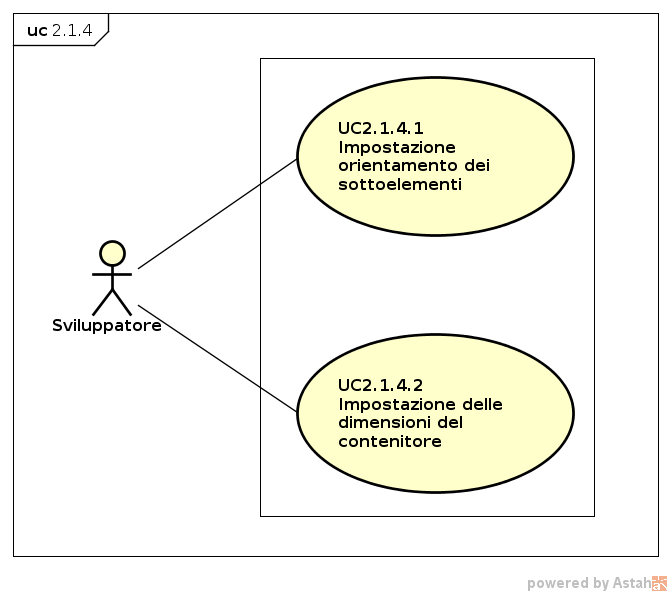
\includegraphics[scale=0.45]{img/UC2_1_4.png}
   \caption{Diagramma per il caso d'uso UC2.1.4.}
\end{figure}
\FloatBarrier
\item[]\textbf{Descrizione:} I contenitori hanno due sole proprietà da modificare: l'allineamento e la dimensione. Ogni contenitore può disporre gli elementi al suo interno accostandoli uno a fianco all'altro oppure impilandoli uno sotto l'altro.


\'E inoltre possibile imporre le dimensioni che il contenitore occupa all'interno del contenitore padre.
\item[]\textbf{Attori:} Sviluppatore. 
\item[]\textbf{Precondizione:} La bolla esiste e include almeno un contenitore. \'E stato selezionato il contenitore da modificare. 
\item[]\textbf{Postcondizione:} \'E stato modificato il valore di una proprietà del contenitore. 
\item[]\textbf{Scenario:}
Lo sviluppatore modifica il valore di una proprietà del contenitore:


\begin{itemize}

\item Impostazione orientamento dei sottoelementi (UC2.1.4.1)

\item Impostazione delle dimensioni del contenitore (UC2.1.4.2)

\end{itemize} 
\end{itemize}

\subsection{Caso d'uso UC2.1.4.1: Impostazione orientamento dei sottoelementi.}
\begin{itemize}
\item[]\textbf{Descrizione:} Viene definito se gli elementi o contenitori contenuti nel contenitore selezionato verranno impilati uno sotto l'altro o se verranno disposti uno a fianco dell'altro. Salvo impostazioni differenti (UC2.1.4.2 e UC2.1.2.1) gli elementi verranno distribuiti equamente nello spazio a disposizione.
\item[]\textbf{Attori:} Sviluppatore. 
\item[]\textbf{Precondizione:} \'E stato selezionato un contenitore. 
\item[]\textbf{Postcondizione:} \'E stato impostato l'orientamento dei sottoelementi. 
\item[]\textbf{Scenario:}
Lo sviluppatore imposta l'orientamento secondo cui dovranno essere disposti i sottoelementi del contenitore selezionato. 
\end{itemize}

\subsection{Caso d'uso UC2.1.4.2: Impostazione delle dimensioni del contenitore.}
\begin{itemize}
\item[]\textbf{Descrizione:} Lo sviluppatore modifica le dimensioni dell'elemento contenitore. Sono possibili due tipi di operazione:

\begin{itemize}

\item in orizzontale la dimensione può essere espressa solo come percentuale sulla dimensione del contenitore padre


\item In verticale la dimensione può essere espressa solo in termini non dipendenti dalla dimensione del contenitore padre


\end{itemize}.
\item[]\textbf{Attori:} Sviluppatore. 
\item[]\textbf{Precondizione:} \'E stato selezionato un contenitore. 
\item[]\textbf{Postcondizione:} \'E stata impostata la dimensione del contenitore. 
\item[]\textbf{Scenario:}
Lo sviluppatore imposta le dimensioni del contenitore 
\end{itemize}

\subsection{Caso d'uso UC2.1.5: Eliminazione contenitore.}
\begin{itemize}
\item[]\textbf{Descrizione:} Viene eliminato il contenitore selezionato. Vengono eliminati anche tutti i contenitori e gli elementi grafici in esso contenuti.
\item[]\textbf{Attori:} Sviluppatore. 
\item[]\textbf{Precondizione:} \'E stato selezionato un contenitore. 
\item[]\textbf{Postcondizione:} Il contenitore selezionato e tutti i suoi discendenti sono stati eliminati. 
\item[]\textbf{Scenario:}
Lo sviluppatore elimina un contenitore precedentemente selezionato e tutti gli elementi o contenitori discendenti da esso. 
\end{itemize}

\subsection{Caso d'uso UC2.1.6: Selezione di elemento grafico o di contenitore.}
\begin{itemize}
\item[]\textbf{Descrizione:} Viene selezionato un elemento grafico o un contenitore. \'E possibile navigare l'albero dei componenti grafici della bolla.
\item[]\textbf{Attori:} Sviluppatore. 
\item[]\textbf{Precondizione:} La bolla è stata creata. 
\item[]\textbf{Postcondizione:} \'E stato selezionato un elemento grafico o un contenitore. 
\item[]\textbf{Scenario:}
Lo sviluppatore accede all'albero dei componenti grafici della bolla e ne seleziona uno. 
\end{itemize}

\subsection{Caso d'uso UC2.1.7: Visualizzazione errore di cancellazione contenitore principale.}
\begin{itemize}
\item[]\textbf{Descrizione:} Viene visualizzato un errore che spiega che non è possibile eliminare il contenitore principale.
\item[]\textbf{Attori:} Sviluppatore. 
\item[]\textbf{Precondizione:} \'E stato selezionato il contenitore principale e si è provato a eliminarlo. 
\item[]\textbf{Postcondizione:} L'eliminazione del contenitore principale è stata impedita. Lo sviluppatore visualizza un messaggio che spiega l'errore. 
\item[]\textbf{Scenario:}
Lo sviluppatore tenta di eliminare il contenitore principale e il sistema glielo impedisce. 
\end{itemize}

\subsection{Caso d'uso UC2.2: Identificazione Mittente o Ricevente.}
\begin{itemize}
\item[]\textbf{Descrizione:} Ciascuna istanza di bolla viene creata da un utente e poi inviata ad uno o più altri utenti. Generalmente ci si aspetta che la bolla si comporti diversamente nelle due situazioni, per esempio fornendo una procedura di inizializzazione al mittente. \'E dunque possibile identificare l'utente corrente come mittente o meno della bolla in esecuzione.
\item[]\textbf{Attori:} Sviluppatore. 
\item[]\textbf{Precondizione:} La bolla esiste. 
\item[]\textbf{Postcondizione:} \'E stata inserita la funzionalità che permette di identificare il mittente. 
\item[]\textbf{Scenario:}
Lo sviluppatore utilizza la funzionalità che permette di identificare a runtime se la bolla è visualizzata dal mittente o da altri utenti. 
\end{itemize}

\clearpage

\subsection{Caso d'uso UC2.3: Gestione del timer.}
\begin{itemize}
   \FloatBarrier
   \begin{figure}[ht]
   \centering
   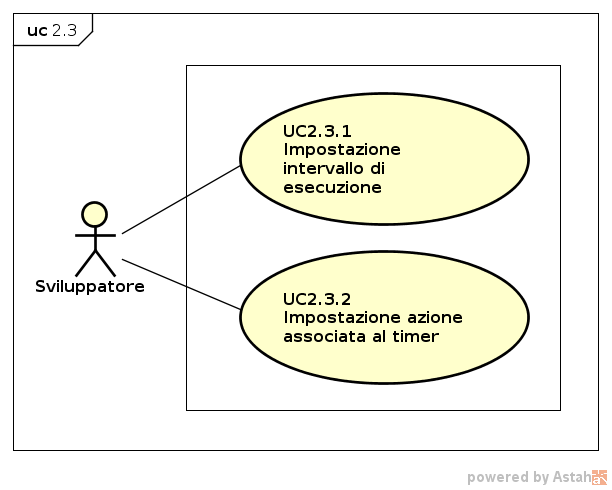
\includegraphics[scale=0.45]{img/UC2_3.png}
   \caption{Diagramma per il caso d'uso UC2.3.}
\end{figure}
\FloatBarrier
\item[]\textbf{Descrizione:} Lo sviluppatore ha la possibilità di impostare  l'esecuzione di azioni automaticamente dopo un certo periodo o con cadenza regolare.
\item[]\textbf{Attori:} Sviluppatore. 
\item[]\textbf{Precondizione:} La bolla esiste. 
\item[]\textbf{Postcondizione:} Nella bolla sono state impostate azioni a tempo. 
\item[]\textbf{Scenario:}
Lo sviluppatore imposta un'azione (UC2.3.2) da eseguire dopo un intervallo prefissato (UC2.3.1.2) oppure a intervalli regolari (UC2.3.1.1) 
\end{itemize}

\clearpage

\subsection{Caso d'uso UC2.3.1: Impostazione dell'intervallo di esecuzione.}
\begin{itemize}
   \FloatBarrier
   \begin{figure}[ht]
   \centering
   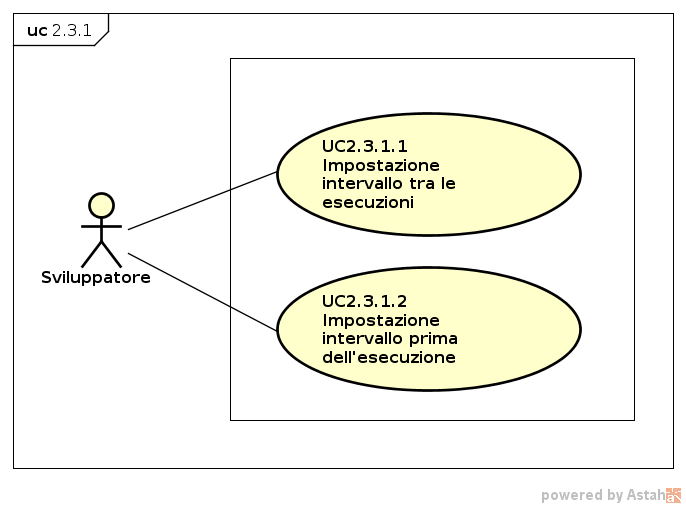
\includegraphics[scale=0.45]{img/UC2_3_1.png}
   \caption{Diagramma per il caso d'uso UC2.3.1.}
\end{figure}
\FloatBarrier
\item[]\textbf{Descrizione:} Viene impostata un'azione da eseguire a intervalli regolari oppure dopo un intervallo prefissato.
\item[]\textbf{Attori:} Sviluppatore. 
\item[]\textbf{Precondizione:} La bolla esiste. 
\item[]\textbf{Postcondizione:} \'E stato impostato l'intervallo prima dell'esecuzione o l'intervallo di ripetizione dell'azione. 
\item[]\textbf{Scenario:}
Lo sviluppatore imposta:

\begin{itemize}

\item l'intervallo tra un'esecuzione e l'altra (UC2.3.1.1)

\item l'intervallo dopo cui eseguire l'azione (UC2.3.1.2)

\end{itemize} 
\end{itemize}

\subsection{Caso d'uso UC2.3.1.1: Impostazione intervallo tra le esecuzioni.}
\begin{itemize}
\item[]\textbf{Descrizione:} Viene impostato ogni quanto tempo eseguire l'azione associata al timer.
\item[]\textbf{Attori:} Sviluppatore. 
\item[]\textbf{Precondizione:} La bolla esiste. 
\item[]\textbf{Postcondizione:} \'E stato impostato l'intervallo di tempo che deve intercorrere tra un'esecuzione e l'altra. 
\item[]\textbf{Scenario:}
Lo sviluppatore imposta l'intervallo tra un'esecuzione e l'altra dell'azione associata al timer 
\end{itemize}

\subsection{Caso d'uso UC2.3.1.2: Impostazione intervallo prima dell'esecuzione.}
\begin{itemize}
\item[]\textbf{Descrizione:} Viene impostato l'intervallo che deve  trascorrere prima di eseguire l'azione associata al timer.
\item[]\textbf{Attori:} Sviluppatore. 
\item[]\textbf{Precondizione:} La bolla esiste. 
\item[]\textbf{Postcondizione:} \'E stato impostato l'intervallo di tempo che deve trascorrere prima di eseguire l'azione associata al timer. 
\item[]\textbf{Scenario:}
Lo sviluppatore imposta l'intervallo di tempo che deve trascorrere prima di eseguire l'azione 
\end{itemize}

\subsection{Caso d'uso UC2.3.2: Impostazione azione associata al timer.}
\begin{itemize}
\item[]\textbf{Descrizione:} Viene impostata l'azione da eseguire in associazione al timer.
\item[]\textbf{Attori:} Sviluppatore. 
\item[]\textbf{Precondizione:} La bolla esiste. 
\item[]\textbf{Postcondizione:} \'E stata associata un'azione al timer. 
\item[]\textbf{Scenario:}
Lo sviluppatore associa un'azione al timer. 
\end{itemize}

\clearpage

\subsection{Caso d'uso UC2.4: Gestione persistenza dei dati.}
\begin{itemize}
   \FloatBarrier
   \begin{figure}[ht]
   \centering
   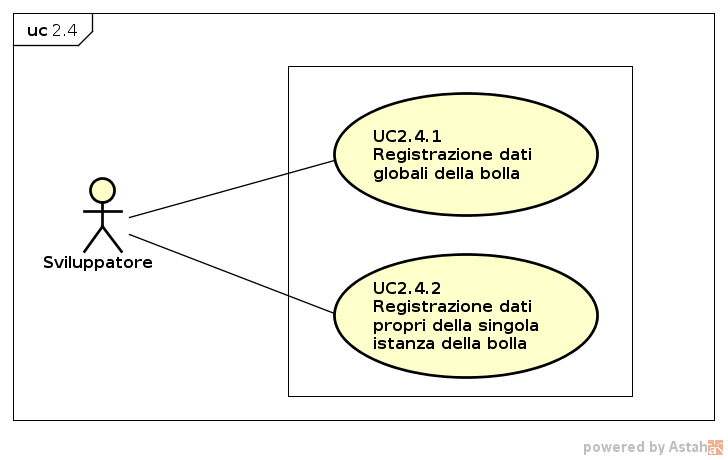
\includegraphics[scale=0.45]{img/UC2_4.png}
   \caption{Diagramma per il caso d'uso UC2.4.}
\end{figure}
\FloatBarrier
\item[]\textbf{Descrizione:} Viene offerta un'interfaccia al sistema di memorizzazione dei dati che fornisca in modo trasparente funzionalità utili allo sviluppo delle bolle. In particolare si permette la distinzione tra dati globali della bolla e dati specifici delle singole istanze.
\item[]\textbf{Attori:} Sviluppatore. 
\item[]\textbf{Precondizione:} La bolla esiste. 
\item[]\textbf{Postcondizione:} \'E stata impostata la persistenza di un'informazione. 
\item[]\textbf{Scenario:}
\begin{itemize}


\item Lo sviluppatore imposta il la persistenza di un'informazione accessibile da ogni istanza della bolla (UC2.4.1)

\item Lo sviluppatore imposta la persistenza di un'informazione propria di una singola istanza della bolla (UC2.4.2)

\end{itemize} 
\end{itemize}

\subsection{Caso d'uso UC2.4.1: Registrazione dati globali della bolla.}
\begin{itemize}
\item[]\textbf{Descrizione:} Viene impostata la persistenza di dati che saranno accessibili da ogni istanza della bolla.
\item[]\textbf{Attori:} Sviluppatore. 
\item[]\textbf{Precondizione:} La bolla esiste. 
\item[]\textbf{Postcondizione:} \'E stata impostata la persistenza di dati validi per tutte le istanze della bolla. 
\item[]\textbf{Scenario:}
Lo sviluppatore imposta la  persistenza di dati che saranno accessibili da ogni istanza della bolla 
\end{itemize}

\subsection{Caso d'uso UC2.4.2: Registrazione dati propri della singola istanza della bolla.}
\begin{itemize}
\item[]\textbf{Descrizione:} Viene impostata la persistenza di dati propri della singola istanza della bolla.
\item[]\textbf{Attori:} Sviluppatore. 
\item[]\textbf{Precondizione:} La bolla esiste. 
\item[]\textbf{Postcondizione:} \'E stata impostata la persistenza di dati propri della singola istanza della bolla. 
\item[]\textbf{Scenario:}
Lo sviluppatore imposta la persistenza di dati propri della singola istanza della bolla 
\end{itemize}

\clearpage

\subsection{Caso d'uso UC0-cv: Bolla convertitore di valuta.}
\begin{itemize}
   \FloatBarrier
   \begin{figure}[ht]
   \centering
   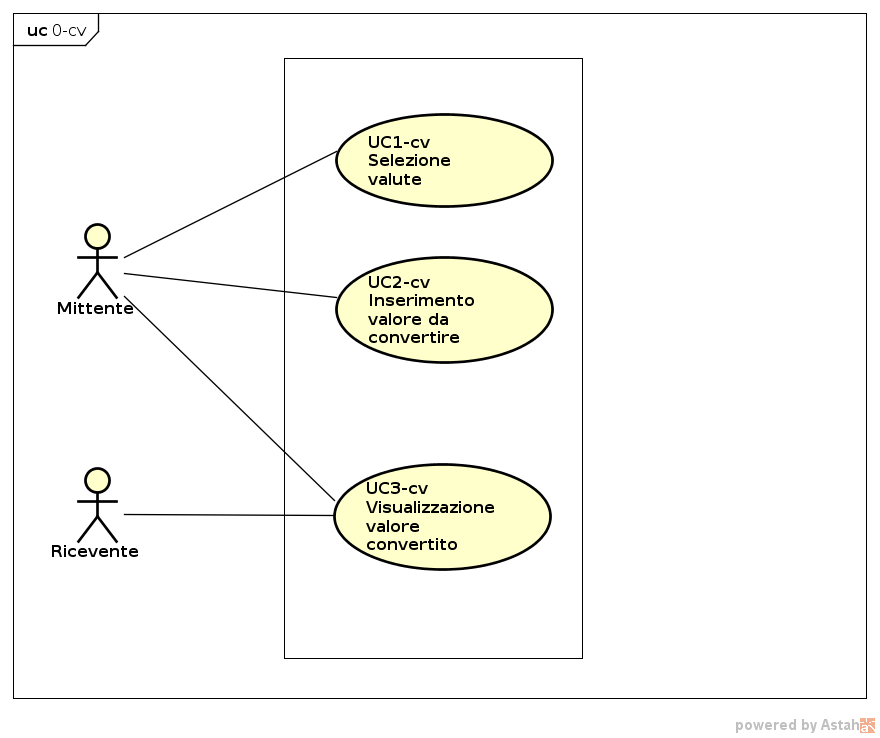
\includegraphics[scale=0.45]{img/soldi.png}
   \caption{Caso d'uso per la bolla di conversione valuta.}
\end{figure}
\FloatBarrier
\item[]\textbf{Descrizione:} La bolla converte gli importi inseriti da una valuta all'altra.
\item[]\textbf{Attori:} Mittente, Ricevente. 
\item[]\textbf{Precondizione:} La bolla è utilizzabile sul sistema del mittente e del ricevente. 
\item[]\textbf{Postcondizione:} La bolla ha convertito l'importo nella valuta di destinazione. 
\item[]\textbf{Scenario:}
\begin{enumerate}


\item Il mittente seleziona la valuta in ingresso e quella in uscita (UC1-cv)

\item Il mittente seleziona un importo da convertire (UC2-cv).

\item Mittente e ricevente visualizzano l'importo convertito (UC3-cv).

\end{enumerate} 
\end{itemize}

\subsection{Caso d'uso UC1-cv: Seleziona valute.}
\begin{itemize}
\item[]\textbf{Descrizione:} Il mittente seleziona la valuta di entrata e quelle di uscita.
\item[]\textbf{Attori:} Mittente. 
\item[]\textbf{Precondizione:} La bolla è utilizzabile sul sistema del mittente e del ricevente. 
\item[]\textbf{Postcondizione:} Le valute sono state selezionate. 
\item[]\textbf{Scenario:}
Il mittente seleziona le valute tra cui effettuare la conversione 
\end{itemize}

\subsection{Caso d'uso UC2-cv: Inserimento importo da convertire.}
\begin{itemize}
\item[]\textbf{Descrizione:} Viene inserito l'importo da convertire.
\item[]\textbf{Attori:} Mittente. 
\item[]\textbf{Precondizione:} Sono state selezionate le valute per la conversione. 
\item[]\textbf{Postcondizione:} L'importo è stato inserito. 
\item[]\textbf{Scenario:}
Il mittente inserisce l'importo da convertire. 
\end{itemize}

\subsection{Caso d'uso UC3-cv: Visualizzazione valore convertito.}
\begin{itemize}
\item[]\textbf{Descrizione:} Vengono visualizzati i valori convertiti.
\item[]\textbf{Attori:} Mittente, Ricevente. 
\item[]\textbf{Precondizione:} Importo e valute sono stati impostati. 
\item[]\textbf{Postcondizione:} L'importo è stato convertito secondo i tassi di cambio richiesti. 
\item[]\textbf{Scenario:}
Il mittente e il ricevente visualizzano i valori convertiti. 
\end{itemize}

\clearpage

\subsection{Caso d'uso UC0-dd: Bolla per l'estrazione di numeri casuali.}
\begin{itemize}
   \FloatBarrier
   \begin{figure}[ht]
   \centering
   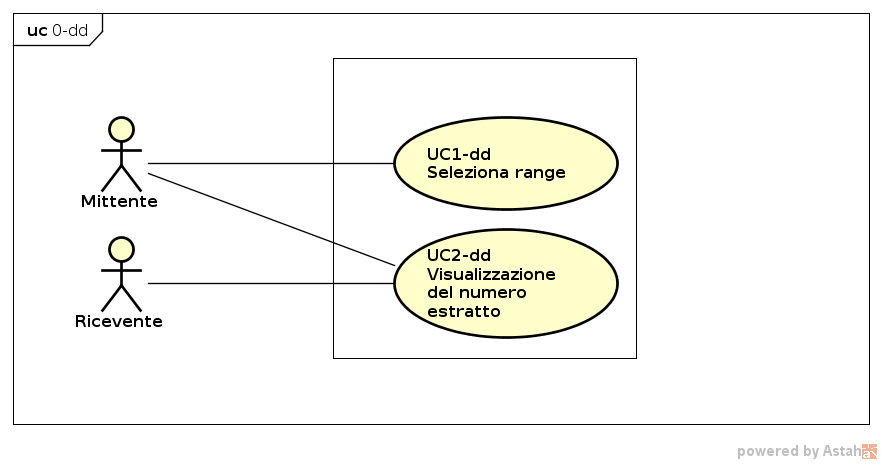
\includegraphics[scale=0.45]{img/random.png}
   \caption{Caso d'uso per la bolla  di estrazione di  numeri casuali}
\end{figure}
\FloatBarrier
\item[]\textbf{Descrizione:} La bolla estrae un numero casualmente dal "range" impostato.
\item[]\textbf{Attori:} Mittente, Ricevente. 
\item[]\textbf{Precondizione:} La bolla è utilizzabile sul sistema del mittente e del ricevente. 
\item[]\textbf{Postcondizione:} La bolla ha restituito un numero scelto casualmente dal "range" impostato. 
\item[]\textbf{Scenario:}
\begin{enumerate}


\item Il mittente seleziona il range da cui estrarre il numero (UC1-dd)

\item Il mittente e il ricevente visualizzano il numero estratto (UC2-dd)

\end{enumerate} 
\end{itemize}

\subsection{Caso d'uso UC1-dd: Seleziona range.}
\begin{itemize}
\item[]\textbf{Descrizione:} Viene selezionato il range da cui estrarre il numero casuale.
\item[]\textbf{Attori:} Mittente. 
\item[]\textbf{Precondizione:} La bolla è installata e funzionante sia sul sistema del mittente che del ricevente. 
\item[]\textbf{Postcondizione:} Il range è stato impostato. 
\item[]\textbf{Scenario:}
Il mittente seleziona il range da cui estrarre il numero 
\end{itemize}

\subsection{Caso d'uso UC2-dd: Visualizzazione numero estratto.}
\begin{itemize}
\item[]\textbf{Descrizione:} Viene visualizzato il numero estratto.
\item[]\textbf{Attori:} Mittente, Ricevente. 
\item[]\textbf{Precondizione:} Il mittente ha selezionato il range e ha inviato la bolla. 
\item[]\textbf{Postcondizione:} Viene mostrato il numero estratto. 
\item[]\textbf{Scenario:}
Il mittente e il ricevente visualizzano il numero estratto 
\end{itemize}

\clearpage

\subsection{Caso d'uso UC0-ls: Lista con checklist.}
\begin{itemize}
   \FloatBarrier
   \begin{figure}[ht]
   \centering
   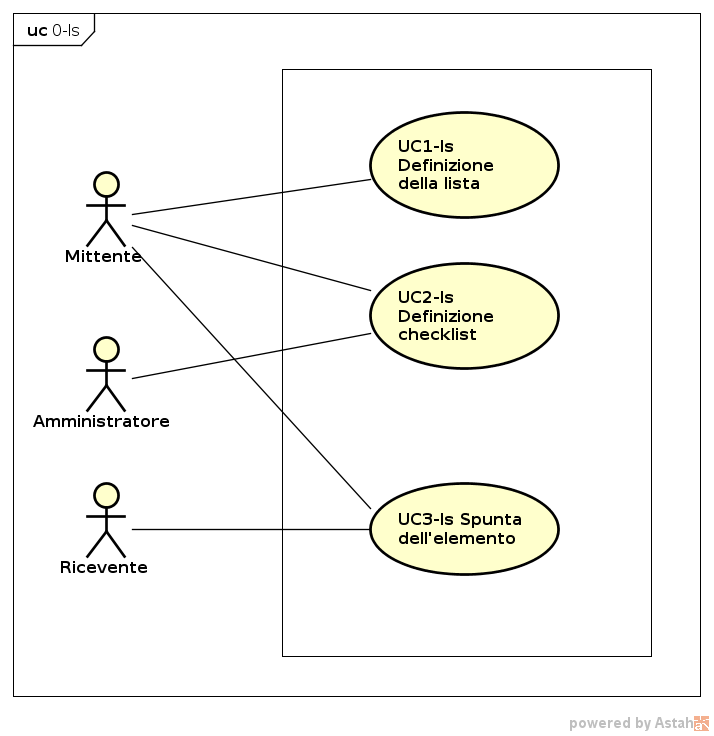
\includegraphics[scale=0.45]{img/lista.png}
   \caption{Caso d'uso per la bolla lista}
\end{figure}
\FloatBarrier
\item[]\textbf{Descrizione:} Il mittente inserisce gli elementi nella lista da inviare, ha inoltre a disposizione una lista di controllo (checklist) da cui prendere elementi. I riceventi possono spuntare elementi dalla lista ricevuta.
\item[]\textbf{Attori:} Mittente, Ricevente, Admin. 
\item[]\textbf{Precondizione:} La bolla è utilizzabile sul sistema del mittente e del ricevente. 
\item[]\textbf{Postcondizione:} Il mittente ha composto e inviato la lista e i riceventi hanno potuto spuntare delle voci. 
\item[]\textbf{Scenario:}
\begin{enumerate}


\item Il mittente definisce la lista da inviare (UC1-ls)

\item Il mittente o l'installatore della bolla definiscono delle checklist predefinite a cui attingere per formare la lista da inviare (UC2-ls).

\item Il ricevente spunta una voce della lista che gli è stata inviata (UC3-ls).


\end{enumerate} 
\end{itemize}

\clearpage

\subsection{Caso d'uso UC1-ls: Definizione della lista.}
\begin{itemize}
   \FloatBarrier
   \begin{figure}[ht]
   \centering
   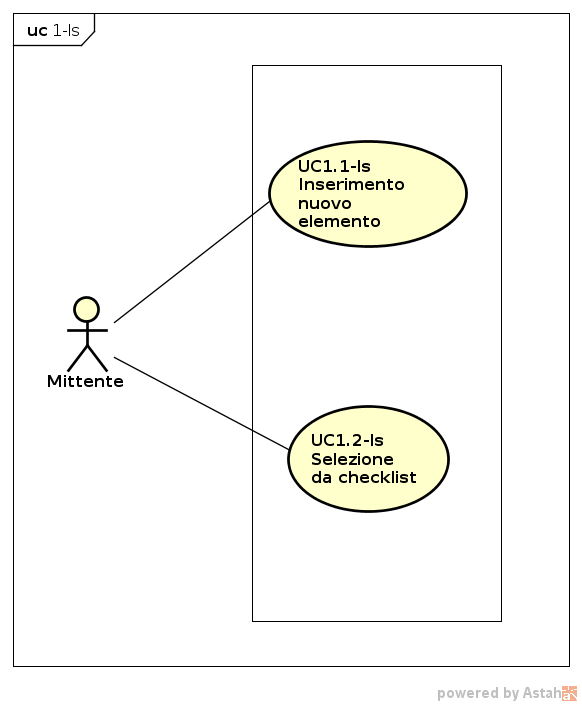
\includegraphics[scale=0.45]{img/lista1.png}
   \caption{Diagramma per il caso d'uso UC1-ls.}
\end{figure}
\FloatBarrier
\item[]\textbf{Descrizione:} Il mittente definisce una lista da inviare.
\item[]\textbf{Attori:} Mittente. 
\item[]\textbf{Precondizione:} La bolla è utilizzabile sul sistema del mittente e del ricevente. 
\item[]\textbf{Postcondizione:} La lista è pronta per essere inviata. 
\item[]\textbf{Scenario:}
\begin{enumerate}


\item Il mittente inserisce un elemento nella lista (UC1.1-ls).

\item Il mittente inserisce un elemento nella lista scegliendolo dalla checklist definita in precedenza (UC1.2-ls).

\end{enumerate} 
\end{itemize}

\subsection{Caso d'uso UC1.1-ls: Inserimento di un nuovo elemento.}
\begin{itemize}
\item[]\textbf{Descrizione:} Il mittente inserisce manualmente un nuovo elemento.
\item[]\textbf{Attori:} Mittente. 
\item[]\textbf{Precondizione:} La bolla è inizializzata ed è pronta per essere configurata. 
\item[]\textbf{Postcondizione:} Una voce è stata inserita nella lista. 
\item[]\textbf{Scenario:}
Il mittente inserisce un elemento nella lista da inviare. 
\end{itemize}

\subsection{Caso d'uso UC1.2-ls: Selezione della voce da checklist.}
\begin{itemize}
\item[]\textbf{Descrizione:} Viene selezionata un voce da una delle checklist da inserire nella lista da inviare.
\item[]\textbf{Attori:} Mittente. 
\item[]\textbf{Precondizione:} La bolla è inizializzata ed è pronta per essere configurata. 
\item[]\textbf{Postcondizione:} Una voce è stata inserita nella lista. 
\item[]\textbf{Scenario:}
Il mittente inserisce un elemento prelevandolo da una lista predefinita 
\end{itemize}

\subsection{Caso d'uso UC2-ls: Definizione di checklist.}
\begin{itemize}
\item[]\textbf{Descrizione:} Viene creata una checklist su cui basare liste future.
\item[]\textbf{Attori:} Mittente, Admin. 
\item[]\textbf{Precondizione:} La bolla è stata installata. 
\item[]\textbf{Postcondizione:} Una checklist è stata creata. 
\item[]\textbf{Scenario:}
Il mittente o l'amministratore della bolla creano una checklist. 
\end{itemize}

\subsection{Caso d'uso UC3-ls: Spunta della voce.}
\begin{itemize}
\item[]\textbf{Descrizione:} Viene spuntata una voce dalla lista ricevuta.
\item[]\textbf{Attori:} Ricevente. 
\item[]\textbf{Precondizione:} Il mittente ha composto e inviato una lista. 
\item[]\textbf{Postcondizione:} Una voce è stata spuntata. 
\item[]\textbf{Scenario:}
Il ricevente spunta una voce dalla lista inviatagli. 
\end{itemize}

\clearpage

\subsection{Caso d'uso UC0-mt: Meteo.}
\begin{itemize}
   \FloatBarrier
   \begin{figure}[ht]
   \centering
   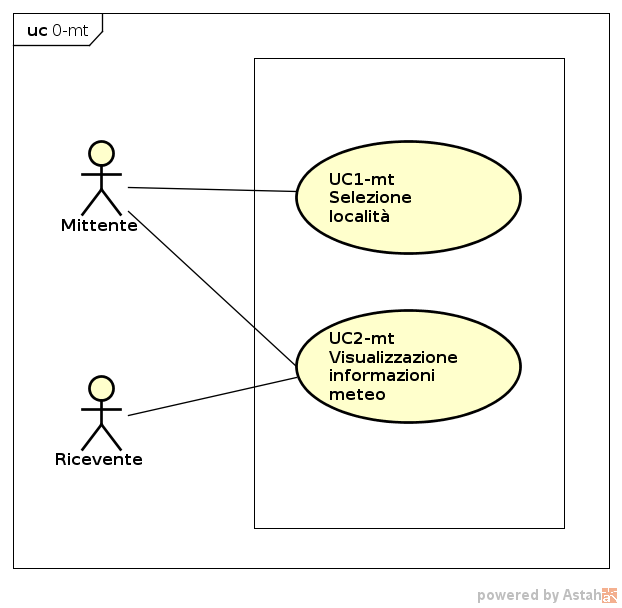
\includegraphics[scale=0.45]{img/meteo.png}
   \caption{Caso d'uso per la bolla meteo}
\end{figure}
\FloatBarrier
\item[]\textbf{Descrizione:} La bolla restituisce le previsioni meteo per la località scelta.
\item[]\textbf{Attori:} Mittente, Ricevente. 
\item[]\textbf{Precondizione:} La bolla è utilizzabile sul sistema del mittente e del ricevente. 
\item[]\textbf{Postcondizione:} La bolla mostra le previsioni meteo per la località scelta. 
\item[]\textbf{Scenario:}
\begin{enumerate}


\item Il mittente seleziona una località (UC1-mt)


\item Il mittente e il ricevente visualizzano le informazioni meteorologiche per la località selezionata (UC2-mt)


\end{enumerate} 
\end{itemize}

\subsection{Caso d'uso UC1-mt: Seleziona località.}
\begin{itemize}
\item[]\textbf{Descrizione:} Viene selezionata la località di cui si desidera visualizzare il meteo.
\item[]\textbf{Attori:} Mittente. 
\item[]\textbf{Precondizione:} La bolla è utilizzabile sul sistema del mittente e del ricevente. 
\item[]\textbf{Postcondizione:} Il mittente ha selezionato la località desiderata. 
\item[]\textbf{Scenario:}
Il mittente seleziona la località desiderata. 
\end{itemize}

\subsection{Caso d'uso UC2-mt: Visualizzazione informazioni meteo.}
\begin{itemize}
\item[]\textbf{Descrizione:} Vengono visualizzate le informazioni meteorologiche richieste.
\item[]\textbf{Attori:} Mittente, Ricevente. 
\item[]\textbf{Precondizione:} Il mittente ha scelto la località desiderata e ha inviato la bolla. 
\item[]\textbf{Postcondizione:} Le informazioni relative alle previsioni meteo sono state visualizzate. 
\item[]\textbf{Scenario:}
Il mittente e il ricevente visualizzano le informazioni meteorologiche richieste. 
\end{itemize}

\clearpage

\subsection{Caso d'uso UC0-sd: Sondaggio.}
\begin{itemize}
   \FloatBarrier
   \begin{figure}[ht]
   \centering
   
\includegraphics[scale=0.45]{img/sondaggio.png}
   \caption{Caso d'uso per la bolla di sondaggio.}
\end{figure}
\FloatBarrier
\item[]\textbf{Descrizione:} Il mittente seleziona un certo numero di opzioni tra cui i riceventi possono scegliere.
\item[]\textbf{Attori:} Mittente, Ricevente. 
\item[]\textbf{Precondizione:} La bolla è utilizzabile sul sistema del mittente e del ricevente. 
\item[]\textbf{Postcondizione:} Il sondaggio si è concluso. 
\item[]\textbf{Scenario:}
\begin{enumerate}


\item Il mittente seleziona le opzioni tra cui è possibile scegliere (UC1-sd).


\item Il mittente può fermare il sondaggio (UC2-sd).


\item I riceventi e il mittente possono scegliere un'opzione da votare (UC3-sd).

\end{enumerate} 
\end{itemize}

\subsection{Caso d'uso UC1-sd: Seleziona opzioni.}
\begin{itemize}
\item[]\textbf{Descrizione:} Vengono impostati un testo introduttivo e le opzioni di voto.
\item[]\textbf{Attori:} Mittente. 
\item[]\textbf{Precondizione:} La bolla è stata selezionata ed è in attesa di essere configurata. 
\item[]\textbf{Postcondizione:} La bolla è stata impostata con i parametri del sondaggio. 
\item[]\textbf{Scenario:}
Il mittente imposta un testo introduttivo e le opzioni di voto. 
\end{itemize}

\subsection{Caso d'uso UC2-sd: Termina sondaggio.}
\begin{itemize}
\item[]\textbf{Descrizione:} Viene interrotto il sondaggio indipendentemente dai voti effettuati.
\item[]\textbf{Attori:} Mittente. 
\item[]\textbf{Precondizione:} Il mittente ha inviato un sondaggio. 
\item[]\textbf{Postcondizione:} Il mittente interrompe il sondaggio. 
\item[]\textbf{Scenario:}
Il mittente impone che il sondaggio termini indipendentemente dai voti effettuati. 
\end{itemize}

\subsection{Caso d'uso UC3-sd: Voto.}
\begin{itemize}
\item[]\textbf{Descrizione:} Vengono espresse le preferenze sulle opzioni proposte.
\item[]\textbf{Attori:} Mittente, Ricevente. 
\item[]\textbf{Precondizione:} Il mittente ha inviato la bolla sondaggio. 
\item[]\textbf{Postcondizione:} L'utente (ricevente o mittente) ha espresso il voto. 
\item[]\textbf{Scenario:}
L'utente (mittente o ricevente) esprime una preferenza tra le opzioni proposte dal mittente. 
\end{itemize}

\subsection{Caso d'uso UC4-sd: Visualizzazione risultati.}
\begin{itemize}
\item[]\textbf{Descrizione:} Vengono visualizzati i risultati della consultazione.
\item[]\textbf{Attori:} Mittente, Ricevente. 
\item[]\textbf{Precondizione:} Il sondaggio è terminato. 
\item[]\textbf{Postcondizione:} I risultati sono stati visualizzati. 
\item[]\textbf{Scenario:}
Il mittente e i riceventi visualizzano i risultati 
\end{itemize}

\clearpage

\subsection{Caso d'uso UC0-tr: Bolla traduttore automatico.}
\begin{itemize}
   \FloatBarrier
   \begin{figure}[ht]
   \centering
   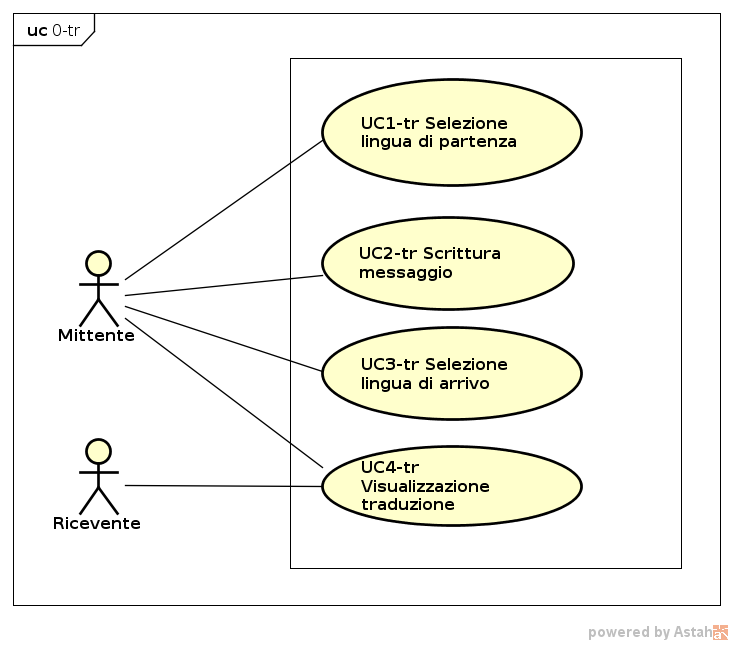
\includegraphics[scale=0.45]{img/traduttore.png}
   \caption{Caso d'uso per la bolla di traduzione}
\end{figure}
\FloatBarrier
\item[]\textbf{Descrizione:} Una bolla che traduce il testo inserito nelle lingue selezionate.
\item[]\textbf{Attori:} Mittente, Ricevente. 
\item[]\textbf{Precondizione:} La bolla è utilizzabile sul sistema del mittente e del ricevente. 
\item[]\textbf{Postcondizione:} Il messaggio viene visualizzato tradotto nella lingua obiettivo. 
\item[]\textbf{Scenario:}
\begin{enumerate}


\item Il mittente seleziona la lingua di partenza (UC1-tr). 

\item Il mittente scrive il messaggio (UC2-tr)

\item Il mittente seleziona la lingua di destinazione (UC3-tr)

\item Mittente e ricevente visualizzano la traduzione(UC4-tr)

\end{enumerate} 
\end{itemize}

\subsection{Caso d'uso UC1-tr: Selezione della lingua di partenza.}
\begin{itemize}
\item[]\textbf{Descrizione:} Viene selezionata la lingua di partenza.
\item[]\textbf{Attori:} Mittente. 
\item[]\textbf{Precondizione:} La bolla è stata selezionata ed è in attesa di essere configurata. 
\item[]\textbf{Postcondizione:} La bolla è configurata con una lingua di partenza. 
\item[]\textbf{Scenario:}
Il mittente seleziona la lingua in cui sarà scritto il messaggio. 
\end{itemize}

\subsection{Caso d'uso UC2-tr: Scrittura del messaggio.}
\begin{itemize}
\item[]\textbf{Descrizione:} Viene inserito il testo del messaggio da tradurre.
\item[]\textbf{Attori:} Mittente. 
\item[]\textbf{Precondizione:} La lingua di partenza è stata configurata. 
\item[]\textbf{Postcondizione:} Il testo del messaggio è stato inserito. 
\item[]\textbf{Scenario:}
Il mittente inserisce il testo del messaggio che deve essere tradotto. 
\end{itemize}

\subsection{Caso d'uso UC3-tr: Selezione lingua di arrivo.}
\begin{itemize}
\item[]\textbf{Descrizione:} Viene selezionata la lingua di arrivo.
\item[]\textbf{Attori:} Mittente. 
\item[]\textbf{Precondizione:} Il testo del messaggio è stato scritto nella lingua di partenza impostata. 
\item[]\textbf{Postcondizione:} La lingua di arrivo è stata impostata. 
\item[]\textbf{Scenario:}
Il mittente seleziona la lingua di arrivo. 
\end{itemize}

\subsection{Caso d'uso UC4-tr: Visualizzazione traduzione.}
\begin{itemize}
\item[]\textbf{Descrizione:} Viene visualizzata la traduzione nella lingua scelta.
\item[]\textbf{Attori:} Mittente, Ricevente. 
\item[]\textbf{Precondizione:} Il testo è stato scritto e le lingue di partenza e di arrivo sono state impostate. La bolla è stata inviata. 
\item[]\textbf{Postcondizione:} \'E stato visualizzato il testo tradotto nella lingua scelta. 
\item[]\textbf{Scenario:}
Il mittente e il ricevente visualizzano la traduzione 
\end{itemize}

